\documentclass[letterpaper, 12 pt, conference]{ieeeconf}
\IEEEoverridecommandlockouts
\overrideIEEEmargins

%---------------- Letter Paper --------------------%
% be sure to change in document class too
\textwidth = 6.9 in
\textheight = 9.0 in
\oddsidemargin = -0.2 in
\evensidemargin = 0.2 in
\topmargin = -0.1 in
%\bottommargin = -0.5 in
\headheight = 0.1 in
\headsep = 0.05in
\parskip = 0.00in
\parindent = 0.1in

% The following packages can be found on http:\\www.ctan.org
\usepackage{graphics}
\usepackage{graphicx}
\usepackage{epsfig}
\usepackage{mathptmx}
\usepackage{times}
\usepackage{amsmath}
\usepackage{amssymb}
\usepackage{siunitx}
\usepackage{multirow}
\usepackage{booktabs}
\usepackage{longtable}
\usepackage{rotating}
\usepackage{textcomp}
\usepackage{bm}
\usepackage{fancyhdr}
\usepackage{comment}
\usepackage{subcaption}
\usepackage{todonotes}
\usepackage{cite}

\title{\LARGE \bf Ragin' Cajuns RoboBoat 2021}
\author{\textbf{Captain}:\\Joseph Stevens \\
\textbf{Members}:\\Nathan Madsen, Brennan Moeller, Adam Smith, Benjamin Willis\\
\textbf{Faculty Advisors}:\\Yasmeen Qudsi and Joshua Vaughan$^{1}$% <-this % stops a space
\thanks{$^{1}$Department of Mechanical Engineering,
        University of Louisiana at Lafayette, Lafayette, LA 70504, USA
        {\tt\small joshua.vaughan@louisiana.edu}}}
 
\bibliographystyle{IEEEtran}
\lhead{\footnotesize{\textit{Ragin' Cajuns RoboBoat}}}
\rhead{\footnotesize{\thepage}}
\cfoot{}
\newpage
\begin{document}\thispagestyle{empty}
\maketitle
\begin{abstract}
This report discusses the design choices and improvements made to the University of Louisiana at Lafayette's first entry in to RoboNation's RoboBoat Competition that includes an Unmanned Aerial Vehicle (UAV). This UAV is to be a mobile sensor for the ASV using its onboard sensors, which include a Real--time Kinematic (RTK) GPS system System, a Raspberry Pi Camera Module, and an OAK--D machine vision sensor. The Ragin' Cajuns RoboBoat is a catamaran-style autonomous surface vessel (ASV) equipped with four thrusters in an ``X"--configuration, enabling holonomic motion. The contributions to the ASV from the 2021 Ragin' Cajuns RoboBoat team include finishing the upgrades to the new electronics enclosure that were hindered due to COVID--19, adding a RTK--GPS system, and upgrading the previous vision sensors to OAK--D machine vision sensors.
\end{abstract}
% 

\section{Introduction}
% 
The 2021 RoboBoat competition requires teams to build an Autonomous Surface Vessel (ASV) capable of performing various tasks that require several subsystems to function together. The ASV shown in Figure~\ref{fig:RoboBoat} is equipped with two planar LiDARs for depth perception, two OAK--D stereo cameras for machine vision feedback, and a~~RTK--GPS and an IMU for localization. The vessel is equipped with four thrusters mounted in an ``X"--configuration, enabling holonomic motion. This vessel is equipped with two Lithium polymer (LiPo) batteries, one 10Ah battery for its thrusters and another 10Ah battery for the electronics. This two battery configuration allows the E-Stops to kill power to thrusters without removing power to the electronics. 

For the 2021 RoboBoat competition, the team added an unmanned aerial vehicle (UAV) to be used as a mobile sensor to assist the ASV in mapping, navigation, and localization. The UAV, shown in Figure~\ref{fig:UAV}, is fitted with an OAK--D machine vision stereo camera to differentiate between the various buoys that will be encountered during the competition and to avoid possible obstacles and a downward--facing Pi Cam to find ArUco markers on top of the ASV's electronics enclosure when landing for object recognition to find pose estimation. It uses RTK--GPS, standard GPS, and an IMU for localization.
% 
\begin{figure}[tb]
\vspace{0.05in}
\centering
\includegraphics[page=2,width=\columnwidth]{TDR/Figures/RoboBoat_Figures.pdf}
\caption{2021 Ragin' Cajuns ASV CAD Model}
\label{fig:RoboBoat}
\end{figure}
% 
It is also equipped with a downward--facing single point LiDAR--Lite for altitude augmentation, an RC receiver for manual flight, and flotation gear to ensure buoyancy. This UAV is powered by one 9.2Ah, 100C discharge rated LiPo battery. The size of the battery was chosen to give an approximate 17 minute flight time. This is a sufficient amount of time for the UAV perform its necessary tasks. If the battery life is detected to be $\le$ 35\%, the UAV will make an emergency landing. The total 2021 Ragin' Cajuns autonomous system is shown in Figure~\ref{fig:complete_system} with its key dimensions highlighted.
% For more information on the exact components in the complete system refer to Table 1 in the Appendix. 
% % 
% \begin{figure}[tb]
% \vspace{0.05in}
% \centering
% \includegraphics[page=2,width=\columnwidth]{TDR/Figures/RoboBoat_Figures.pdf}
% \caption{2021 Ragin' Cajuns ASV CAD Model}
% \label{fig:RoboBoat}
% \end{figure}
% % 
\begin{figure}[tb]
\vspace{0.09in}
\centering
\includegraphics[page=3,width=\columnwidth]{TDR/Figures/RoboBoat_Figures.pdf}
\caption{2021 Ragin' Cajuns UAV CAD Model}
\label{fig:UAV}
\end{figure}
% 
\begin{figure}[tb]
\vspace{0.13in}
\centering
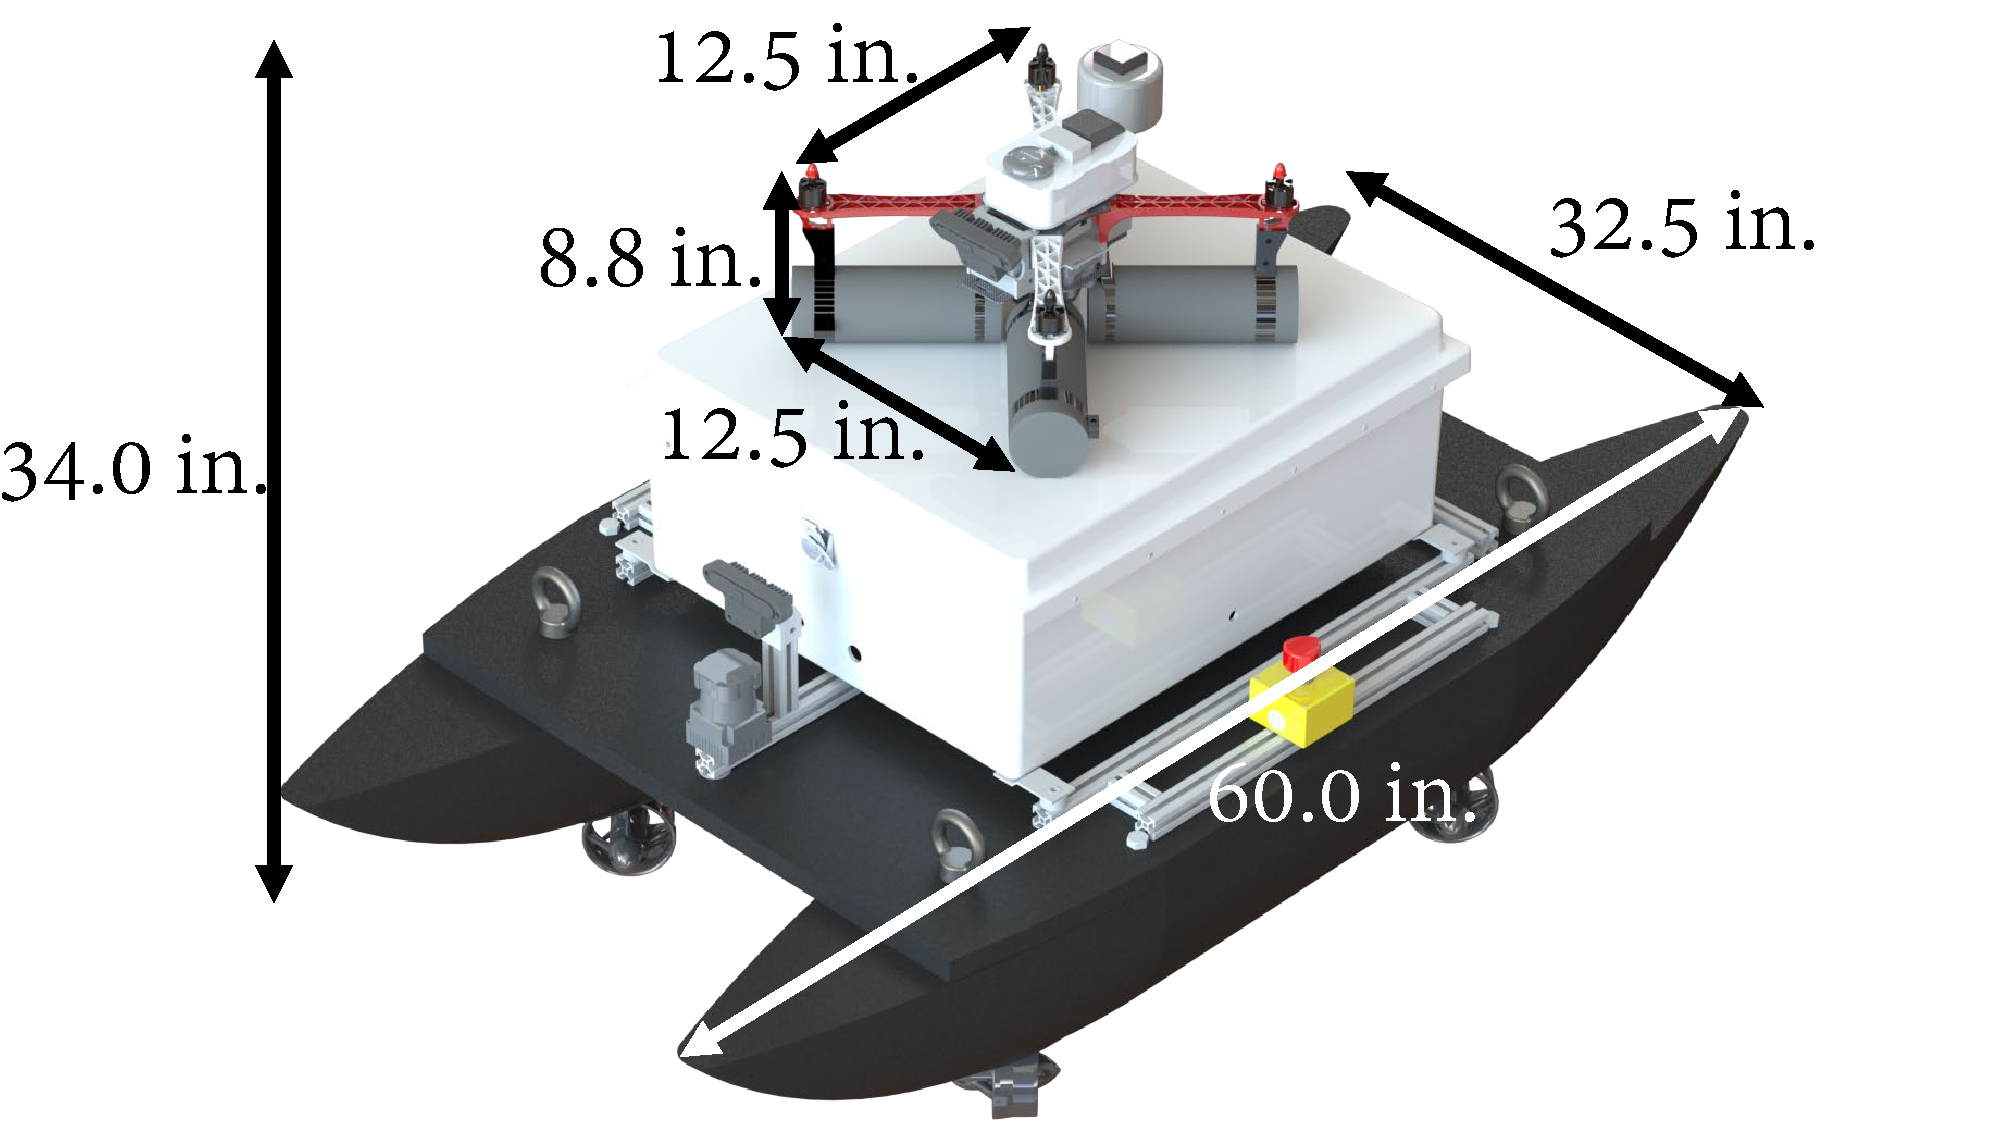
\includegraphics[page=1,width=\columnwidth]{TDR/Figures/RoboBoat_Figures.pdf}
\caption{2021 Ragin' Cajuns Autonomous System}
\label{fig:complete_system}
\end{figure}
% 

In the next section, the competition strategy for the 2021 competition is discussed. The design creativity of the ASV and the new UAV are discussed in Section III. In Section IV, the experimental results that were gathered are presented. Finally, Section V is the conclusion. A list of components is also presented in the Appendix.
% 

\pagestyle{fancyplain} 
\section{Competition Strategy}
% 
The past competitions have shown that the Ragin' Cajuns ASV is an adaptable and capable vessel for RoboBoat's challenges. However, there was room for improvements including utilizing a UAV in the competition, upgrading localization and sensing components, and improving the control architecture of the system. This year, integrating a UAV and upgrading the localization of the system were selected as the main foci. The following sections will discuss the strategic approach for the UAV integration and how the system will operate in the competition.
% 
\subsection{UAV Integration} 
% total approximate of 6,050 points. 
Through an analysis of the past competitions, it was determined that the team could potentially obtain an approximate 1,200 additional points by adding a UAV that takes off of and lands on the ASV, and completes the UAV--specific task. The addition of a UAV to the current ASV requires tight integration of software and mechanical design. To facilitate the integration of the UAV's and ASV's sensing, mapping, perception, and controls, the Robot Operating System (ROS) is used. To ensure the designed UAV could be integrated to the ASV, computer--aided design (CAD) models of the UAV and ASV were created and updated throughout the process. While this integration increased the complexity of the system, the ASV can operate independently of the UAV, allowing for each run to continue even if the UAV fails. 

For the 2021 competition, the UAV will be deployed after the mandatory Navigation Channel is completed and move to the next section of the course. This allows the UAV to be one task ahead of the ASV to collect data and place waypoints for the ASV to navigate to. 
% This UAV uses a PX4 Flight Management Unit (FMU) and a Raspberry Pi 4 Model B as its companion computer. These computational devices allow for easy integration to the ASV due to their easy implementation of the ROS framework.
% 
\subsection{System Software}
% 
A mix of custom and standard ROS packages are used for the control, perception, and mapping. The $robot$\_$localization$ package is used both on the ASV and UAV. It combines GPS and IMU sensor data, pose estimates from $rtabmap$\_$ros$, and ArUco markers to compute a single state estimation of each system \cite{MooreStouchKeneralizedEkf2014}. The global loop-closure Simultaneous Localization and Mapping (SLAM) package, $rtabmap$\_$ros$, uses the data collected from the OAK--D stereo cameras and the planar LiDARs on the ASV, as well as the  OAK--D on the UAV to create 3D point cloud maps \cite{Rtabmap}. The maps created by the UAV and ASV are compiled into a single map using a ROS package called $multirobot\_map\_merge$, which allows multiple maps from different robots to be compiled into one map \cite{multirobotmap}. ArUco markers allow for the pose of a camera to be determined from a square marker that is similar to a quick response (QR) square \cite{Aruco}. The ASV electrical enclosure lid is fitted with an ArUco marker array. This gives the UAV a more accurate pose estimation when landing on the ASV.

ROS is also used to aid in the overall communication of data for the system by allowing multiple peripherals to share information across computers connected to the network. as shown in Figure~\ref{fig:Network}. The 2.4 GHz sector, or antenna, creates a networking bridge from the on shore router to the access point on the ASV. This access point also gives the UAV access to the network. Figure~\ref{fig:ROSGraph} is a high--level overview of the ROS network for this system, which allows all the information gathered from both the ASV's and UAV's sensors to be shared. For example, the $mavros$ package is used to communicate with the flight controller on the UAV and publishes the data to the ROS master that it is recording \cite{mavros}.
% 
\begin{figure}[tb]
\vspace{0.09in}
\centering
\includegraphics[page=39,width=\columnwidth]{TDR/Figures/RoboBoat_Figures.pdf}
\caption{2021 Ragin' Cajuns Network}
\label{fig:Network}
\end{figure}
% 
\begin{figure}[tb]
\vspace{0.13in}
\centering
\includegraphics[page=40,width=\columnwidth]{TDR/Figures/RoboBoat_Figures.pdf}
\caption{Graph of ROS Network}
\label{fig:ROSGraph}
\end{figure}
% 

Due to the volume of information that is being collected and processed, multiple computational devices are needed. Furthermore, the imagine processing tasks that are required for this competition are best handled by dedicated Graphics Processing Units (GPUs). For this reason two Jetson TX2s are used on the ASV. These devices are used for image processing and mapping. The ASV also has one Raspberry Pi 4 Model B that handles basic sensor reading and lower--level thruster control. The UAV uses a Raspberry Pi 4 Model B as the companion computer for its Pixhawk 4 flight controller.

To speed up configuration, initialization, and booting, Docker was used to create containers that could be implemented on multiple devices \cite{merkel2014docker}. A Docker container contains all of the dependencies, packages, system tools, and settings needed to execute an application. This allows the same container to be run on different operating systems, such as the operating systems contained in the two TX2s or the two Raspberry Pis. Docker also allows the code that is needed to execute certain tasks to be mounted to the container at time of use. This allows the code to be saved to a platform like GitHub, so the development can be split across a team \cite{roboboatgit}. 
% %
\begin{figure*}[t]
\centering
\includegraphics[page=23,width=1.65\columnwidth]{TDR/Figures/RoboBoat_Figures.pdf}
\caption{State Machine for the UAV in the Obstacle Channel Task}
\label{fig:UAVObstacleChan}
\end{figure*}
% %
% % % 
% \begin{figure*}[t]
% \centering
% \vspace{0.05in}
% \includegraphics[page=23,width=1.75\columnwidth]{TDR/Figures/RoboBoat_Figures.pdf}
% \caption{State Machine for the UAV in the Obstacle Channel Task}
%     \vspace{-3ex}
% \label{fig:UAVObstacleChan}
% \end{figure*}
% % %
\subsection{Navigation Channel}
\label{NavigationChannel}
% 
Completing the Navigation Channel task is mandatory and must be done before attempting any other tasks in the competition. The complete system must pass through two sets of gates consisting of two buoys at least six feet apart. The two sets of gates are at least 50 feet apart. The Ragin' Cajuns RoboBoat system is equipped with forward facing stereoscopic cameras on both the UAV and ASV that provide images to a “You Only Look Once” (YOLOv3) Convolution Neural Network (CNN), object detection in real time \cite{DBLP:journals/corr/abs-1804-02767}. The training set for this CNN consists of manually-labeled images from the 2019 competition, as well as images from the 2016 Maritime RobotX Competition. The output of the image classifier is passed to a state machine that determines how the ASV or UAV should maneuver.

For the Navigation Channel task, the state machine directs the ASV to find a gate, identified with green in the right side of the frame and red in the left. A waypoint goal to maneuver to the middle of the gate and orient the vessel to be in--line with the channel is sent to the navigation stack. The state machine instructs the ASV to maintain the initial heading as it continues to drive forward and look for the exit gate. Another waypoint between the exit gate buoy is sent to the navigation stack as a target location. Once the exit gate is found, and the vessel reaches this waypoint, it completes the Navigation Channel and prepares to launch the UAV. Furthermore, if the UAV cannot find the exit gate it will continue to the next provided GPS location, and the ASV's peripherals will guide it through the channel. 
% % %
% \begin{figure*}[t]
% \centering
% \includegraphics[page=23,width=1.65\columnwidth]{TDR/Figures/RoboBoat_Figures.pdf}
% \caption{State Machine for the UAV in the Obstacle Channel Task}
% \label{fig:UAVObstacleChan}
% \end{figure*}
% % %
\subsection{Obstacle Channel}
\label{ObstacleChannel}
% 
The Obstacle Channel requires the ASV to maneuver through a series of gates with obstacle buoys along the trajectory. Unlike the Navigation Channel, these gates are arranged in a non--linear path. This task may be difficult to complete because of the ASV's relatively large footprint. However, the holonomic thruster configuration allows the ASV to exert forces and moments in each degree of freedom independently increasing its maneuverability. Furthermore, it is equipped with a RTK--GPS system to help improve localization. This increased maneuverability, increased localization precision, and data collected by the UAV helps the Ragin' Cajuns RoboBoat complete this task.

Once the ASV exits the Navigation Channel, the UAV launches, hovers, and then is tasked with finding the Obstacle Channel via GPS coordinates and object recognition. An outline of the UAV's state machine for the Obstacle Channel is shown in Figure~\ref{fig:UAVObstacleChan}. The state $back\_to\_launching$ is invoked if the UAV cannot launch for any reason. Similarly, a redundancy is in place if the UAV cannot find the obstacle channel. There is a limit to the number of times a redundancy state can be entered; stopping the UAV from entering a continuous loop. If this limit is reached for any state other than launching the UAV it will then continue to the next task's GPS location and begin surveying. If the UAV reaches this limit during the launching process, it will send a a message to a computer on shore and reboot its companion computer and reinitialize the state machine. Once the UAV finds the Obstacle Channel, it uses the CNN to follow the channel, similar to how the Navigation Channel was identified, green in the right side of the frame and red in the left. The UAV places waypoints approximately in the middle of the channel as it flies above. This information is available for the ASV through the ROS network. 

Once the ASV arrives at this task, it utilizes the map that was created by the UAV with its path planning package, $roboboat\_navigation$. This allows the ASV to have an understanding of its environment and a desired path to follow through the channel before it arrives at the task. The vision feedback system provided to the navigation stack prevents the ASV from colliding with the green, red, and yellow buoys.
% It will be looking for green buoys in the right side of the image and red buoys in the right to identify the gates. The vision feedback system provided to the navigation stack will prevent the ASV from colliding with these green and red buoys as well as the yellow obstacle buoys. Waypoints are recursively placed at the middle of the gates. In order to know that the task has been completed, the GPS coordinate for the Obstacle Field task is iteratively appended to the waypoint sequence. When no more gates are in the field of view, the ASV will begin maneuvering to the Obstacle Field task because this waypoint is the last in the sequence. If red and green buoys in the Obstacle Field are misinterpreted as gates, the path planner will prevent the ASV from entering a region that it cannot fit because it knows the base footprint area.
% This task requires the ASV to localize a signal and dock in its location. The state machine behaviors for this task are shown in Figure \ref{fig:AcousticDocking}. Once the Navigation Channel task has been successfully completed, the state machine instructs the ASV to maneuver to the GPS coordinate provided for the entrance to the Acoustic Docking task, avoiding potential obstacles along the way. Once the ASV arrives at the docking station, two hydrophones are deployed from the vessel's stern using a linear actuator. The ASV then circumnavigates the dock to generate a map of the area.  Hydrophone feedback is processed to localize the active acoustic beacon and record its location. Once the signal has been located, if the docking station is not in view, the state machine will prescribe a waypoint away from the dock and instruct the ASV to adjust its heading to see the circle, cruciform, or triangle symbol associated with the recorded location. This symbol is identified using the image classifier and recorded, as it may affect the tasks that follow. The recorded location of the active acoustic beacon is then used as a waypoint to maneuver back to the dock. When the ASV has reached the target location, docking will commence. The ASV will station keep in the dock for five to ten seconds to confirm that it has successfully docked, and then exit the dock by setting the GPS coordinates for the Obstacle Channel task as its next waypoint.
\subsection{Obstacle Field}
\label{ObstacleField}
% 
Once the UAV exits the Obstacle Channel, it moves to the Obstacle Field to create a map for the ASV to use. The UAV uses the GPS coordinate and the CNN to determine the location of the Obstacle Field on this course. It will identify the pill buoy by using the YOLOv3 CNN to determine if the pill buoy is in the frame. Then, the UAV circumnavigates this buoy while updating the distances between the buoys to find the largest entrance and place a waypoint at that location. 

When the ASV reaches the Obstacle Field, it moves towards the opening specified by the UAV. The ASV saves the location of the entrance and enters. Next, the path planner uses the map created by $multirobot\_map\_merge$ to plan a trajectory around the pill buoy. Once the pill buoy has been circled, and the ASV has changed its heading by at least 360 degrees, the ASV will exit the Obstacle Field using the recorded position as the last waypoint and head towards the Speed Gate task. 
% 
% This task is attempted immediately after the Obstacle Channel task. The state machine behaviors for this task are shown in Figure \ref{fig:ObstacleField}. The Obstacle Field task is similar to the Obstacle Channel, but instead of gates, there is one ``Pill Buoy", which has distinguished markings, that the ASV must circumnavigate. This buoy is surrounded by several obstacles spaced as little as four feet apart. The Ragin' Cajuns RoboBoat team's approach to this task is handled by collaboration between the high-level state machine and the path planner. The state machine will determine that the ASV is at the Obstacle Field by first identifying the Pill Buoy in the cameras' field of view. The state machine will then place a waypoint toward the Pill Buoy to motivate the ASV to approach it. An entrance to the Obstacle Field is found by circumnavigating the field of buoys, iteratively updating the largest distance identified between the adjacent buoys. The path planner will then plan a trajectory through the obstacles while maintaining a safe distance from obstacles that is manually prescribed. This value is chosen as smaller than 50\% of the difference between the minimum specified distance between obstacles the ASV can pass through, four feet, and the beam width of the Ragin' Cajuns RoboBoat. When the ASV has entered the Obstacle Field the current position is recorded, the state machine will command the path planner to circumnavigate the obstacle by placing waypoints around it. Once the Pill Buoy has been circled, and the ASV has changed its heading by at least 360$^\circ$, the ASV will exit the Obstacle Field using the recorded position as the last waypoint  and locating of a pair of buoys the computer vision system and path planner find wide enough for the ASV to fit.
\subsection{Speed Gate}
\label{SpeedGate}
% 
After the UAV finishes mapping the Obstacle Field, the GPS coordinates are sent to the navigation stack to motivate the ASV to move toward that location. As it approaches, the CNN is used to locate the one standalone gate that consists of one green and one red buoy. The UAV then hovers and looks for the marker buoy, a single blue buoy. Once the buoy is found, the UAV places a waypoint at the gate and flies toward the blue buoy where it places another waypoint. 

Once the ASV completes the Obstacle Field, it proceeds toward the waypoint that was placed at the entrance of the speed gate by the UAV. The state machine overrides the velocity restrictions that were in place for the earlier tasks where speed was not a priority, so this task can be completed as quickly as possible. Then, the state machine instructs the ASV to pass through the gate at maximum speed. Once the target buoy has been located, waypoints are placed around it so it can be circumnavigated. The initial position at the gate is used as the final waypoint to guide the ASV out of the Speed Gate Challenge. 
% After the obstacle field has been successfully escaped, the ASV will maneuver to the GPS coordinate provided for the Speed Gate entrance. This task introduces a race element to the competition. The ASV is required to enter through a gate, travel to a buoy and circle it, and return through the gate as quickly as possible. Because of the new enclosure that was procured for this competition, the ASV thrust-to-weight ratio has decreased, hurting our possible performance at this task. However, the new optimal control strategy implemented for this year's competition may be more effective than the velocity controller used at the previous competition. Additionally, the state machine overrides the velocity restrictions placed on the ASV by the path planner for this task so it can be completed as quickly as possible. A waypoint is placed at the gate entrance, and then the state machine instructs the ASV to pass through the gate at maximum speed. Once the target buoy has been located, waypoints are placed around it to it can be circumnavigated. The initial position at the gate is used as the final waypoint to guide the ASV out of the Speed Gate Challenge.
% 
\subsection{Return to Dock}
\label{ReturnToDock}
% 
Once the UAV has finished all of the tasks, it will then fly towards the ASV, guided by their shared localization data. As it approaches the vessel, the downward facing Pi Cam identifies an ArUco tag array that is on top of that ASV's enclosure, as shown in Figure~\ref{fig:aruco}. These markers are used to determine the UAV's location in reference to the ASV. Then, the UAV follows the ASV to the starting position and prepares to land.

After the ASV finishes the Speed Gate challenge, it navigates back to the starting location that was recorded upon entering the course. Throughout the competition, the ASV was creating a map of the course. This map is used to guide it back to the starting position while avoiding any of the obstacles or exiting the course. Once the ASV reaches the dock, it holds its position to allow the UAV to land on top of it. With the Pi Cam's estimation, the increased accuracy of the RTK--GPS system, and the LiDAR--Lite altitude augmentation, the UAV will slowly approach the lid of the enclosure and land.

%After the ASV finishes the Speed Gate challenge, it navigates back to the starting location that was recorded upon entering the course. Throughout the competition, the ASV was creating a map of the course by recording all of the obstacles' location and features. Along with the ASV's localization and path planning capabilities, this map is used to maneuver it back to the starting position without encountering any of the obstacles or exiting the course. Once the ASV reaches the dock, it holds its position with the help from its navigation stack to allow for the UAV to land on top of it. With the Pi Cam's estimation and the increased accuracy of the RTK--GPS system, the UAV will slowly approach the lid of the enclosure. Once the UAV is approximately 4 in from the lid of the enclosure, the UAV will land.  


% Once all other tasks have been completed, the final task the ASV can complete is returning to the starting point of the course without encountering any obstacles and having the UAV land on top of the ASV. The ASV must pass through its own course, and not another where other vessels are competing. This is accomplished by recording the starting position upon entering the water, and then upon completing the final competition task, activating that saved location as a waypoint. While the ASV is completing other competition tasks, it will also be generating a map of the environment. In conjunction with its localization and path planning capabilities, this will be used to maneuver the ASV back to the starting dock.
%
\begin{figure}[tb]
\vspace{0.05in}
\centering
\includegraphics[page=30,width=\columnwidth]{TDR/Figures/RoboBoat_Figures.pdf}
\caption{ArUco Markers On Top of ASV to Aid UAV in Landing}
\label{fig:aruco}
\end{figure}
%
\subsection{Acoustic Docking}
% 
The Acoustic Docking task requires the vessel to localize a docking signal and dock itself in the specified docking bay. The 2021 Ragin' Cajuns RoboBoat team declined to continue to develop upon the previous system used for this task. The focus was on to the design, manufacture, and integration of the UAV to the ASV system.
% 
\subsection{Object Delivery}
\label{ObjectDelivery}
% 
The Object Delivery task requires the ASV to deliver up to four objects to a specified area in the course. The task may be completed solely by the ASV or by a combination of an ASV and UAV. The 2021 Ragin' Cajuns RoboBoat team declined to develop the required mechanism to complete this task. However, the frame selection and custom frame plates for the UAV that were designed with additional mounting holes allowing for future development.

% Should a task like this be introduced in future competitions, the Ragin' Cajuns RoboBoat would have been tasked with collecting images of the new course elements to enhance the image classifier training set, which currently has a limited supply of dock-like images.

\section{Design Creativity}
\subsection{Thrust Configuration}
% 
The thrusters are mounted to the hull of the ASV in a ``X"--configuration, mounted at $45^\circ$ angles relative to the bow. A free--body diagram of this thruster configuration is shown in Figure \ref{fig:FBD}.
%
\begin{figure}[tb]
\centering
\includegraphics[page=4,width=\columnwidth]{TDR/Figures/RoboBoat_Figures.pdf}
\caption{Free-Body Diagram of RoboBoat Thruster Configuration}
\label{fig:FBD}
\end{figure}
This configuration enables holonomic motion, or motion in all three degrees of freedom independent of each other. This improves the maneuverability of the ASV, which is especially valuable in tasks like the Obstacle Channel and Obstacle Field.
%Though this thrust configuration was used on the past Ragin' Cajuns RoboBoat entry, its performance has shown that for this system it is still sufficient. 

Furthermore, the addition of the RTK--GPS system, that receives RTCM (Radio Technical Commission for Maritime-services) data to increase the accuracy of standard GPS signals to centimeter levels, improves the precision of the ASV's localization \cite{RTKLIB}. This specific thruster configuration allows the ASV to take full advantage of the increased localization precision.


% Though this thrust configuration was used on the 2019 Ragin' Cajuns entry to the competition, the design was only equipped with one stereo camera and LiDAR. This meant that there was a $90^\circ$ region that no visual measurements were being taken, so it was possible that, with a mapping error, the 2019 RoboBoat would apply reverse or sway thrust and encounter an obstacle. Because the 2021 design has two LiDAR systems and stereo cameras, the blind spot is removed. 
%
\subsection{UAV Center of Mass}
% 
Throughout the design of the UAV, component placement was driven by the effects that the location and mass of the components would have on the COM of the UAV. The location of the COM in reference to the horizontal plane in which the rotors lie has an affect on both the stability of forward flight and the UAV's ability to combat wind disturbances \cite{compaper}. For this application, a COM below the horizontal plane in which the rotors lie is desirable, because it increases forward flight stability. In its current state, the location of the UAV's COM, relative to the center of the horizontal plane in which the rotors lie, is (-0.025, -2.163, -0.010) in, as shown in Figure \ref{fig:com}. 
% As previously stated, the UAV's desired COM drove the placement, mount design, and selection of the components.
%
\begin{figure}[tb]
\vspace{0.05in}
\centering
\includegraphics[page=5,width=\columnwidth]{TDR/Figures/RoboBoat_Figures.pdf}
\caption{UAV Center of Mass}
\label{fig:com}
\end{figure}
\subsection{UAV Enclosures}
% 
The RoboBoat competition takes place regardless of weather conditions. Therefore, it is imperative to keep all electronics safe from rain water. This is achieved by fully enclosing them in 3D printed enclosures. These enclosures are also used to directly mount the electronics to the UAV. It was determined that all enclosures must meet Ingress Protection (IP) 34 standards, water resistant from splashes of water in all directions \cite{IP}. 

The main electronics enclosure for the UAV, shown in Figure~\ref{fig:MainElct}, is made of acrylonitrite butadiene styrene (ABS) because of its UV and weather resistant properties. The main electronics in this enclosure are a Pixhawk 4 Flight Control Unit (FCU) and a Raspberry Pi 4 companion computer as shown in Figure~\ref{fig:MainElct}. Further considerations were made to ensure other electronics be protected from water ingress such as the Pi Cam, RTK--GPS, and power module. The LiDAR--Lite V3HP equipped on the UAV already exceeded the desired qualifications with an IPX7 rating.
% 
\begin{figure}[tb]
\centering
\includegraphics[page=35,width=\columnwidth]{TDR/Figures/RoboBoat_Figures.pdf}
\caption{Main UAV Electronics Enclosure and Mount}
\label{fig:MainElct}
\end{figure}
% 
To ensure that the main electronics would not overheat or result in CPU throttling, a heat transfer analysis was completed. The problem is modeled as a thermal resistance problem, as seen in Figure~\ref{fig:HeatTransfer}.
% 
\begin{figure}[tb]
\centering
\includegraphics[page=15,width=\columnwidth]{TDR/Figures/RoboBoat_Figures.pdf}
\caption{Model of Simple Heat Transfer Problem}
\label{fig:HeatTransfer}
\end{figure}
%
The hottest temperature that Florida has ever reached is $T_{1}$, $43^{\circ}$C, and $T_{2}$, $71^{\circ}C$, represents the average operating temperature of a Raspberry Pi, which is 20-30$^{\circ}$C above the ambient operation temperature \cite{FloridaHot,PiHOT}. This calculation determined that the system would dissipate heat to the environment through the enclosure, but more importantly that the Raspberry Pi's CPU would operate approximately 16.5\% under its throttling temperature, 85$^{\circ}$C. 

% $T_{1}$ represents that hottest temperature that Florida has ever reached and

% % 
% \begin{figure}[tb]
% \centering
% \vspace{0.05in}
% \includegraphics[page=15,width=\columnwidth]{TDR/Figures/RoboBoat_Figures.pdf}
% \caption{Model of Simple Heat Transfer Problem}
%     \vspace{-3ex}
% \label{fig:HeatTransfer}
% \end{figure}
% % 

% %
% \begin{figure}[tb]
% \centering
% \includegraphics[page=9,width=\columnwidth]{TDR/Figures/RoboBoat_Figures.pdf}
% \caption{Main UAV Electronics Enclosure}
% \label{fig:MainEncl}
% \end{figure}
% %
% %
% \begin{figure}[tb]
% \centering
% \includegraphics[page=10,width=\columnwidth]{TDR/Figures/RoboBoat_Figures.pdf}
% \caption{Main UAV Electronics Mount}
% \label{fig:MainElct}
% \end{figure}
% %
%
% \begin{figure}[tb]
% \centering
% \includegraphics[page=35,width=\columnwidth]{TDR/Figures/RoboBoat_Figures.pdf}
% \caption{Main UAV Electronics Enclosure and Mount}
% \label{fig:MainElct}
% \end{figure}
% %
% \subsection{UAV Enclosures}
% % 
% Being that the RoboBoat competition will happen regardless of weather conditions it was imperative to keep all of the electronics safe. This was achieved by fully enclosing them in 3D printed enclosures. These enclosures would also be used to directly mount the electronics to the UAV. It was determined that all enclosures must meet Ingress Protection (IP) 34 standards. This results in them being water resistant from splashes of water in all directions. To ensure that the main electronics would not overheat or be introduced to unnecessary throttling, simple heat transfer calculations were done. The problem was modeled as a simple thermal resistance problem, as seen in Figure~\ref{fig:HeatTransfer}. $T_{1}$ represents that hottest temperature that Florida has ever reached and $T_{2}$ represents the average operation temperature of Raspberry Pi which is 20-30$^{\circ}$C above the ambient operation temperature \cite{FloridaHot,PiHOT}. This calculation determined that the system would dissipate heat to environment through the enclosure, but more importantly that the Raspberry Pi's CPU would not reach its throttling temperature, 85$^{\circ}$C. The main enclosure would be made of acrylonitrite butadiene styrene (ABS) because of its UV and weather resistant properties shown in Figure~\ref{fig:MainEncl}. In Figure~\ref{fig:MainElct}, the main electronics in this enclosure include a Pixhawk 4 Flight Control Unit (FCU) and a Raspberry Pi 4 companion computer. Further considerations were made to ensure other electronics be protected from water ingress such as the Raspberry Pi Camera Module V2, RTK--GPS, and power module. The LiDAR Lite V3HP equipped on the UAV already exceeded the desired qualifications with an IPX7 rating. The mountings for these enclosures were driven by the COM considerations that were previously discussed. 
% These were tested by placing water absorbing material inside each of these enclosures, then, spraying water to all angles of the enclosures. All enclosures passed the required testing. 
% %
% \begin{figure}[tb]
% \centering
% \vspace{0.05in}
% \includegraphics[page=15,width=\columnwidth]{TDR/Figures/RoboBoat_Figures.pdf}
% \caption{Model of Simple Heat Transfer Problem}
%     \vspace{-3ex}
% \label{fig:HeatTransfer}
% \end{figure}
%
% \subsection{UAV Landing Gear \& Flotation Device}
% % 
% The 2021 RoboBoat rules require that any UAV that is used in the competition be positively buoyant. This is a difficult challenge to achieve for a UAV that is being modified for data collection due to the additional weight added by the sensors. Another challenge is ensuring that the device does not obstruct the flow of air to the rotors. Three designs were considered including spheres on the feet of the frame, a square tube around the perimeter of the UAV, and cylindrical tubes in an ``X" configuration under the UAV. These designs each had advantages and disadvantages; however, the chosen design, due to its ease of assembly, least air flow obstruction, and its ability to be adjusted, was the cylindrical tubes in ``X" configuration, as seen in Figure~\ref{fig:FloatGear}. The cylindrical tubes used are industrial, polyethylene backer rods. This flotation device is also suitable for landing the on ASV or solid ground.
% % %
% \begin{figure}[tb]
% \centering
% \includegraphics[page=19,width=\columnwidth]{TDR/Figures/RoboBoat_Figures.pdf}
% \caption{UAV Flotation/Landing Gear}
% \label{fig:FloatGear}
% \end{figure}
% % %
\subsection{Data Acquisition}
% 
\subsubsection{Raspberry Pi Camera Module V2}
% 
A Pi Cam was positioned on the bottom plate of the UAV to be used as a downward facing image sensor to collect data for object detection and landing procedures. In Figure \ref{fig:picamfov}, a sketch showing the analysis of the horizontal field of view (FOV), 62.2 degrees, of the PiCam can be seen. A small amount of the polyethylene foam is in the camera's FOV. However, this amount of interference was later determined to be insignificant.

%As with all components added to the UAV, multiple design challenges had to be overcome with a creative approach to ensure proper component placement. These challenges included affects on the COM, mount design to minimize weight, and placement to reduce the interference with other components.

%This shows a successful design insuring correct measures be taken to avoid FOV interference by the flotation device.

%The horizontal, not the vertical, FOV was considered due to it having the larger FOV, accounting for the maximum available FOV.
\begin{figure}[tb]
\centering
\includegraphics[page=21,width=\columnwidth]{TDR/Figures/RoboBoat_Figures.pdf}
\caption{Raspberry Pi Camera Module V2 FOV}
\label{fig:picamfov}
\end{figure}

%With the UAV designed to land back on the enclosure, and the design of the flotation device
\subsubsection{OAK--D FOV}
% 
An OAK--D stereo camera will be used by the UAV to capture distance and RGB image data for purposes of mapping, object detection, and obstacle avoidance. As seen in Figure~\ref{fig:oakdfov}, the vertical FOV of the OAK--D stereo camera is 56 degrees. The forward facing camera mount which holds the OAK--D on the UAV is designed with a 20 degrees angle from the vertical, as seen in Figure~\ref{fig:cammount}. This angle gives the OAK--D the capability of capturing image data above and below the horizontal plane providing data for both obstacle avoidance and object recognition, respectively. This mount also locks the cameras position on the UAV allowing for the exact location to be known when the camera is collecting data.
%
\begin{figure}[tb]
\centering
\includegraphics[page=20,width=\columnwidth]{TDR/Figures/RoboBoat_Figures.pdf}
\caption{OAK--D Field of View}
\label{fig:oakdfov}
\end{figure}
%
%
\begin{figure}[tb]
\centering
\includegraphics[page=8,width=\columnwidth]{TDR/Figures/RoboBoat_Figures.pdf}
\caption{OAK--D Camera Mount for UAV}
\label{fig:cammount}
\end{figure}
%

To keep the implementation of code across the system uniform, the ASV's stereoscopic sensors were upgraded to OAK--D machine vision sensors. The OAK--D machine vision sensor was added to both bow and stern adding a 72 degrees RGB FOV. This allows the ASV to take full advantage of its holonomic motion capabilities. Similar to the UAV, the mounting brackets for these cameras allow for their exact position to be known when they are collecting data.
% %
% \begin{figure}[tb]
% \centering
% \includegraphics[page=34,width=\columnwidth]{TDR/Figures/RoboBoat_Figures.pdf}
% \caption{OAK--D Camera Mount for ASV}
% \label{fig:asvoakmount}
% \end{figure}
% %
% \subsubsection{Real-time Kinematic-GPS System}
% % 
% Due to the lowering costs and geometrical constraints on Real-time Kinematic (RTK) GPS systems, it was determined that integrating an RTK system was necessary for the addition of this UAV. This addition would require the AS
\subsubsection{Planar LiDARs}
% 2
The ASV is also equipped with two Hokuyo planar LiDARs for obstacle avoidance and mapping. These LiDARs are positioned in the middle of the ASV on both the bow and stern and offer a wider FOV than the OAK-D's RGB and depth sensing FOVs, as seen in Figure~\ref{fig:ASVLiDAR}. They give the ASV an approximate 230 degrees FOV of its surroundings, front and rear, thus increasing its ability to utilize its holonomic motion. These LiDAR sensors also give the ASV an approximate 64.8\% increase in horizontal perception from only having stereo vision.
%
\begin{figure}[tb]
\centering
\includegraphics[width=\columnwidth]{TDR/Figures/ASV_fieldOfView_gray_v4_Adobe Devanagari.pdf}
\caption{ASV LiDAR FOV}
\label{fig:ASVLiDAR}
\end{figure}
%
\section{Experimental Results}
% 
% The experimental tests that were conducted for this system include both physical and simulated experiments. The UAV was integrated into the RotorS Micro Air Vehicle (MAV) Gazebo simulator \cite{rotors:2016}. This simulation allows the ROS packages and scripts that are needed for the perception sensors and mapping algorithms on the UAV to be tested. Physical tests on the system included testing buoyancy, the IP rating of the electronics enclosures, and the RTK--GPS accuracy for the Ragin' Cajuns RoboBoat system. 
% Both simulated and real world experiments were ran on the ASV/UAV system. The simulated experiments were done in a physics based environments to ensure realistic testing. The UAV flight controller was tuned both in simulation and physically. The UAV in the real world was able to lift off an fly to different heights under its own power and the ASV was able to be tested in a swamp with its new autopilot controller, NAVIO2. 
\subsection{System Simulation}
% 
Models of the ASV and the UAV were developed for use in the $rotors\_simulator$ ROS package because of its use of a physics--based ROS application called Gazebo \cite{inproceedings}, \cite{rotors:2016}. Each sensor that is on the UAV can also be simulated, such that the FOV and data being collected represent that of the actual sensor.

In this simulated environment, all of the sensors were configured to accurately represent their specifications. In RotorS, flight paths can be set, scripts that control the perception and mapping algorithms can be executed, and data can be collected. For example, Figure~\ref{fig:RViz} shows depth data collected by the simulated OAK--D stereo camera on the left and RGB image data collected by the simulated OAK--D digital camera on the top right. The bottom right image in Figure~\ref{fig:RViz} displays RGB image data collected by the simulated Pi Cam. This simulation also allows for safer testing during future development of the UAV.
% 
\begin{figure}[tb]
\vspace{0.05in}
\centering
\includegraphics[page=3,width=\columnwidth]{TDR/Figures/RViz.png}
\caption{UAV Peripheral Simulation in RViz}
\label{fig:RViz}
\end{figure}
%
% \subsubsection{Gazebo}
% The biggest contribution of this team to the continued development of the Ragin' Cajuns RoboBoat is the foundation for a system simulation in Gazebo. The RoboBoat spawns in the Sand Island World from the Virtual Maritime RobotX Competition \cite{Bingham:19a}, shown in Figure \ref{fig:YOLO}.
% %
% \begin{figure}[tb]
% \centering
% \vspace{0.05in}
% \includegraphics[width=\columnwidth]{Figures/YOLOV3.png}
% \caption{Testing the RoboBoat Image Classifier in Sand Island}
% \label{fig:YOLO}
% \end{figure}
% %
% Here, the image classifier training is being tested on its ability to recognize the buoys. The classifier uses ``You Only Look Once" (YOLOv3) \cite{Redmon:18a}, trained using the CNN described in Section \ref{NavigationChannel}. The simulation is based on the Heron Simulation from Clearpath Robotics \cite{Bogdon:19a}. The ROS network on-board the RoboBoat computer systems and sensors has been migrated to generic, configurable sensors with open-source plugins to simulate data such as point clouds, laser scans, and wind and wave effects. 

% The ACADO toolkit is used to generate a MPC controller \cite{Houska:11a}. Several other nodes are used to perform localization or act as components in the ROS Navigation Stack. The current configuration still needs lots of tuning, but the 2020 Ragin' Cajuns RoboBoat team decided that focusing on developing this platform as a tool for future competitions would be the best course of action.
\subsection{Buoyancy Test for the UAV}
%
To ensure the UAV's flotation device was properly designed, testing was conducted in a controlled environment. The completely loaded system was placed in a controlled body of water to validate the buoyancy calculations as seen in Figure~\ref{fig:FloatTesting}. Figure~\ref{fig:Underwater} shows the submerged amount of the flotation device was approximately half of the cylinder, 1.5in. This result validates the preliminary analysis which showed that the cylinders needed to have approximately $\frac{2}{3}$ of their volume submerged in water. 
% %
% \begin{figure}[tb]
% \centering
% \includegraphics[page=38,width=\columnwidth]{TDR/Figures/RoboBoat_Figures.pdf}
% \caption{Submerged Flotation/Landing Gear}
% \label{fig:Underwater}
% \end{figure}
% % 
%As seen in Figure~\ref{fig:FloatTesting}, the UAV does float.
\begin{figure}[tb]
\vspace{0.05in}
\centering
\includegraphics[page=26,width=\columnwidth]{TDR/Figures/RoboBoat_Figures.pdf}
\caption{Testing of Flotation Device in Controlled Environment}
\label{fig:FloatTesting}
\end{figure}
% 
%
\begin{figure}[tb]
\centering
\includegraphics[page=27,width=\columnwidth]{TDR/Figures/RoboBoat_Figures.pdf}
\caption{Submerged Flotation/Landing Gear}
\label{fig:Underwater}
\end{figure}
% 
% With a completed CAD model, the team would like to verify the hand calculations for the convection heat transfer from the enclosure surface and perform thermal analyses within the enclosure itself. Though it is not ready for this year's competition, the updated CAD model will be used to generate these system characteristics before the 2021 competition, and may result in further hardware upgrades such as an air circulation system to be included within the enclosure.
% \subsection{IP Rating Test}
% 
% Since the UAV's electronics enclosures were designed to approximate IP34 standards, a simulated test was conducted to ensure ingress protection from water. The test was conducted by first adding a piece of a hydrophilic material within the enclosures to make any water ingress visible. Next, a water bottle was modified to spray the enclosures. The results for the main electronics enclosure are displayed in Figure~\ref{fig:IPTestResults}. With the test results showing no water ingress, the design approximations of IP34 standards were satisfied.
% %
% \begin{figure}[tb]
% \vspace{0.05in}
% \centering
% \includegraphics[page=28,width=\columnwidth]{TDR/Figures/RoboBoat_Figures.pdf}
% \caption{Approximate IP34 Standard Test Results}
% \label{fig:IPTestResults}
% \end{figure}
% % 
\subsection{RTK Accuracy} 
% 
To increase the localization accuracy of the UAV and ASV, Real--time Kinematic (RTK) positioning was used. A typical RTK system can achieve centimeter--level accuracy, as apposed to a standard GPS, which has roughly 16ft. of radial error. The accuracy associated with an RTK system is a function of time and the number of satellites and base stations in the area. The RTK system for the Ragin' Cajuns RoboBoat consists of one base station that has a fixed location on shore and stations on each of the autonomous systems. A test was done to see what accuracy could be achieved in a 10--minute time frame. As seen in Figure~\ref{fig:RTK}, in under 9 minutes, the system's radial error was reduced to 6 feet. The system did not reach its full potential of centimeter level accuracy, but increasing the run time of the RTK system would allow improved accuracy to be achieved. Moreover, the RTK--GPS system was tested throughout this year. On average, the RTK--GPS system's error would decrease between 1.5--2ft after approximately 4--6 hours. During this time, the number of visible satellites was 17--20.
%
\begin{figure}[tb]
\vspace{0.05in}
\centering
\includegraphics[page=29,width=\columnwidth]{TDR/Figures/RoboBoat_Figures.pdf}
\caption{RTK Accuracy with QGround Control}
\label{fig:RTK}
\end{figure}
% 
\subsection{System Test} 
% 
Once the Ragin' Cajuns RoboBoat System was completed, it was taken to a local pond to run some general tests on the system's new components including the new navigation stack, as well as testing the manoeuvrability of the ASV with its new enclosure mounted. In Figure~\ref{fig:systemTest}, the system is on the water and general testing was being conducted on the operation of the system. Unfortunately, during the test, a thruster mount broke and hit the side of the ASV causing a small divot in the hull, as shown in Figure~\ref{fig:brokenthrust}. Plans to fix the hull, mount, and finish tuning the UAV's controller are scheduled before the June 13th deadline for the Optional Operational Video. 
%
\begin{figure}[tb]
\vspace{0.05in}
\centering
\includegraphics[page=32,width=\columnwidth]{TDR/Figures/RoboBoat_Figures.pdf}
\caption{System Testing}
\label{fig:systemTest}
\end{figure}
% 
%
\begin{figure}[tb]
\vspace{0.05in}
\centering
\includegraphics[page=33,width=\columnwidth]{TDR/Figures/RoboBoat_Figures.pdf}
\caption{Malfunction During Testing}
\label{fig:brokenthrust}
\end{figure}
% 
%
\section{Conclusions}
% 
This paper presented the design of the 2021 Ragin' Cajuns RoboBoat system, including key software, hardware, and strategic improvements. This design builds on the Ragin' Cajuns' 2019 and 2020 entries into the RoboBoat contest and now includes a UAV to aid in data collection, upgraded ~OAK--D~ machine vision sensors, and a RTK--GPS system for increased improved accuracy. Contributions made by this team to furthering the Ragin' Cajuns RoboBoat development at the University of Louisiana at Lafayette include a Gazebo simulation of the UAV, an updated CAD model of both systems, and a platform to attempt more tasks in the future, including the Object Delivery task. The upgrades to the sensors and the addition of the UAV by this team will be useful to future Ragin' Cajuns RoboBoat teams.
% 
% This report analyzed the design of the 2020 Ragin' Cajuns RoboBoat, including key software, hardware, and strategic improvements. This design builds on the Ragin' Cajunss' previous entry to the RoboBoat Challenge, and now utilizes Model Predictive Control, an optimal control strategy. The sensor configuration that the RoboBoat is equipped with now eliminates a blind spot that limited the usefulness of the holonomic thruster configuration. Contributions made by this team to furthering ASV development at the University of Louisiana at Lafayette include a Gazebo simulation of the RoboBoat system and an updated CAD model. Competition strategies employed and documented by this team may serve useful to future Ragin' Cajuns RoboBoat team members.
% 
\section{Acknowledgments}
% 
The 2021 team would like to thank Chapman Consulting Inc. for allowing us access to their facilities and resources. Also, the team would like to thank Microsoft Azure and Intel for sponsoring the OpenCV OAK--D AI Competition which allowed us to win 10 free OAK--D machine vision sensors.

\bibliography{Citations.bib}

\onecolumn
\begin{appendix}
\begin{center}
\begin{longtable}{lccccc}
\caption{Ragin' Cajuns RoboBoat Specifications}\\
\label{SpecSheet}
\textbf{Category} & \textbf{Item} & \textbf{Vendor}& \textbf{Specifications} & \textbf{Quantity} & \textbf{Price (\$)}\\
\hline
Battery & 4S Li-Po & Turnigy & \begin{tabular}{c}16V\\ 5200 mAh \\ 450g \end{tabular} & 4 & 53.96\\
\\
Battery & 3S Li-Po & Floureon & \begin{tabular}{c}12V \\ 4500 maH \\ 324.5g \end{tabular} & 2 & 33.29\\
\\
Battery & 3S Li-Po & Zeee & \begin{tabular}{c}12V, 100C \\ 9000 maH \\ 560g \end{tabular} & 2 & 71.00\\
\\
Comm. & TL-WA901ND & TP-Link & \begin{tabular}{c} 2.4-2.4835 GHz \\ 270m range \\ 12V, 1A \\ 5.8W\end{tabular} & 1 & 37.99\\
\\
Computing &  \begin{tabular}{c}Raspberry Pi 4\\Model B\end{tabular} & \begin{tabular}{c} ARMv8, 1.5 Ghz \\ 8GB DDR4 RAM\end{tabular} & 2 & 90.00\\
\\
Computing & Jetson TX2 & NVIDIA & \begin{tabular}{c} 256 CUDA Cores \\ 2-Core Denver 2 \\ 4-Core Cortex-A57\\8GB DDR4 RAM  \end{tabular} & 2 & 629.99\\
\\
Control & NAVIO2 HAT & EMLID & \begin{tabular}{c} 5V, 150 mA \\ Cortex-M3 \\ IMU, Barometer  \end{tabular} & 1 & 168.00\\
\\
Control & PX4 FMU & Holybro & \begin{tabular}{c} 5V\\ 2 Accel/Gryo\\ Barometer \\  \end{tabular} & 1 & 245.00\\
\\
Enclosure & PJ24208RT & \begin{tabular}{c}Hammond\\MFG\end{tabular} & \begin{tabular}{c} 0.064 $\text{m}^3$ \\ Fiberglass \\ 11 kg \end{tabular} & 1 & Donated\\
\\
\end{longtable}
\end{center}
\onecolumn
\begin{center}
\begin{longtable}{lccccc}
\caption{Ragin' Cajuns RoboBoat Specifications Cont.}\\
\label{SpecSheet}
\textbf{Category} & \textbf{Item} & \textbf{Vendor}& \textbf{Specifications} & \textbf{Quantity} & \textbf{Price (\$)}\\
\hline
Hull & \begin{tabular}{c}Fiberglass\\Cloth\end{tabular} & TotalBoat & 6 $\frac{\text{oz}}{\text{yard}^2}$ & 10.56 $\text{yard}^2$ & 56.01\\
\\
Hull & Epoxy & TotalBoat & 1.18 $\frac{\text{g}}{\text{cm}^3}$ & 4.31 kg & 126.99\\
\\
Hull & \begin{tabular}{c}Fairing\\Compound\end{tabular} & TotalBoat & 1.32 $\frac{\text{g}}{\text{cm}^3}$ & 2.27 kg & 56.99\\
\\
Propulsion & T-200 & \begin{tabular}{c}Blue\\Robotics\end{tabular} & \begin{tabular}{c} $\left[-4.1, 5.25\right]$ kgf \\ 76mm Propeller \\ 156g (in water) \\ 390W, 24A (max)\end{tabular} & 4 & 169.00\\
\\
Propulsion  & \begin{tabular}{c}Speed\\Controllers\end{tabular} & \begin{tabular}{c}Blue\\Robotics\end{tabular}  & \begin{tabular}{c}16.3g \\ 7--26V \\ 30A (max) \\$\left[1100,1900\right]$ $\mu$s\end{tabular} & 8 & 25.00\\
\\
Propulsion & \begin{tabular}{c}MT 2213 Motor\\1045 Propeller \end{tabular}& \begin{tabular}{c}EMAX \end{tabular} & \begin{tabular}{c} 935KV, 860g thrust \\ 1045 Propeller\end{tabular} & 4 &  67.00\\
\\
Sensing & \begin{tabular}{c}GPS-RTK \\Board \end{tabular} & SparkFun & \begin{tabular}{c} 5V, 35mA \\ 5Hz-RTK\\ NEO-M8P-2 \end{tabular} & 3 & 199.95\\
\\
Sensing & \begin{tabular}{c}LiDAR Lite\\V3 HP\end{tabular} & Garmin & \begin{tabular}{c} 1m-40m, 5V \\ 85mA\end{tabular} & 1 & 150.00 \\
\\
Vision & UTM-30-LX-EW & Hokuyo & \begin{tabular}{c} $270^\circ$ FOV \\ 2D Projection \\ 30 meter range \\ 100 Hz \end{tabular} & 2 & 4900.00\\
\\
Vision & \begin{tabular}{c}Camera \\ Module V2 \end{tabular}& \begin{tabular}{c} Raspberry Pi \end{tabular} & \begin{tabular}{c} 8 MP \\ Sony IMX219 \\ $62.2^\circ$, $48.8^\circ$\end{tabular} & 2 & 25.00\\
\\
Vision & \begin{tabular}{c}OAK--D\\Stereo Camera \end{tabular}& \begin{tabular}{c}Luxonis \\ OpenCV \end{tabular} & \begin{tabular}{c} 1MP \\ 1280x800 120 FPS\\  900mA / 5V \\ 115g \\ $81^\circ$, $71.8^\circ$\end{tabular} & 2 & Won\\
\end{longtable}
\end{center}
\onecolumn
\begin{center}
\begin{longtable}{lccccc}
\caption{Ragin' Cajuns RoboBoat Specifications Cont.}\\
\label{SpecSheet}
\textbf{Category} & \textbf{Item} & \textbf{Vendor}& \textbf{Specifications} & \textbf{Quantity} & \textbf{Price (\$)}\\
\hline
Vision & \begin{tabular}{c}OAK--D\\RGB Camera \end{tabular}& \begin{tabular}{c}Luxonis \\ OpenCV \end{tabular} & \begin{tabular}{c} 12MP \\ 4@K30 FPS \\  900mA, 5V \\ 115g \\ $81^\circ$, $68.8^\circ$\end{tabular} & 2 & Won\\
\\
Frame & \begin{tabular}{c}F450\\Quad-rotor \end{tabular}& \begin{tabular}{c}DJI \end{tabular} & \begin{tabular}{c}450mm footprint\end{tabular} & 1 & 72.00\\
\\
\end{longtable}
\end{center}
\end{appendix}
\end{document}